% Set up the document
\documentclass[a4paper, 12pt, oneside]{Thesis} 

%%------------------------------------HEADER FILE
\graphicspath{Figures/}  % Location of the graphics files (set up for graphics to be in PDF format)

% Include any extra LaTeX packages required
\usepackage[square, numbers, comma, sort&compress]{natbib}  % Use the "Natbib" style for the references in the Bibliography
\usepackage{verbatim}  % Needed for the "comment" environment to make LaTeX comments
\usepackage{vector}  % Allows "\bvec{}" and "\buvec{}" for "blackboard" style bold vectors in maths
\hypersetup{urlcolor=blue, colorlinks=true}  % Colours hyperlinks in blue, but this can be distracting if there are many links.

\usepackage{sectsty}
\chapterfont{\centering}




%Define the listing package
\usepackage{listings} %code highlighter
\usepackage{color} %use color
\definecolor{mygreen}{rgb}{0,0.6,0}
\definecolor{mygray}{rgb}{0.5,0.5,0.5}
\definecolor{mymauve}{rgb}{0.58,0,0.82}
\definecolor{dkgreen}{rgb}{0,0.6,0}
\definecolor{gray}{rgb}{0.5,0.5,0.5}

%Customize a bit the look
\lstset{ %
backgroundcolor=\color{white}, % choose the background color; you must add \usepackage{color} or \usepackage{xcolor}
basicstyle=\footnotesize, % the size of the fonts that are used for the code
breakatwhitespace=false, % sets if automatic breaks should only happen at whitespace
breaklines=true, % sets automatic line breaking
captionpos=b, % sets the caption-position to bottom
commentstyle=\color{mygreen}, % comment style
deletekeywords={...}, % if you want to delete keywords from the given language
escapeinside={\%*}{*)}, % if you want to add LaTeX within your code
extendedchars=true, % lets you use non-ASCII characters; for 8-bits encodings only, does not work with UTF-8
frame=single, % adds a frame around the code
keepspaces=true, % keeps spaces in text, useful for keeping indentation of code (possibly needs columns=flexible)
keywordstyle=\color{blue}, % keyword style
% language=Octave, % the language of the code
morekeywords={*,...}, % if you want to add more keywords to the set
numbers=left, % where to put the line-numbers; possible values are (none, left, right)
numbersep=5pt, % how far the line-numbers are from the code
numberstyle=\tiny\color{mygray}, % the style that is used for the line-numbers
rulecolor=\color{black}, % if not set, the frame-color may be changed on line-breaks within not-black text (e.g. comments (green here))
showspaces=false, % show spaces everywhere adding particular underscores; it overrides 'showstringspaces'
showstringspaces=false, % underline spaces within strings only
showtabs=false, % show tabs within strings adding particular underscores
stepnumber=1, % the step between two line-numbers. If it's 1, each line will be numbered
stringstyle=\color{mymauve}, % string literal style
tabsize=2, % sets default tabsize to 2 spaces
title=\lstname % show the filename of files included with \lstinputlisting; also try caption instead of title
}
%END of listing package%
 
\definecolor{darkgray}{rgb}{.4,.4,.4}
\definecolor{purple}{rgb}{0.65, 0.12, 0.82}
 
%define Typescript language
\lstdefinelanguage{TypeScript}{
keywords={typeof, new, true, false, catch, function, return, null, catch, switch, var, if, in, while, do, else, case, break },
keywordstyle=\color{blue}\bfseries,
ndkeywords={class, export, boolean, throw, implements, import, this},
ndkeywordstyle=\color{purple}\bfseries,
identifierstyle=\color{mygreen},
sensitive=false,
comment=[l]{//},
morecomment=[s]{/*}{*/},
commentstyle=\color{purple}\ttfamily,
stringstyle=\color{red}\ttfamily,
morestring=[b]',
morestring=[b]"
}
 
\lstset{frame=tb,
  language=TypeScript,
  aboveskip=3mm,
  belowskip=3mm,
  showstringspaces=false,
  columns=flexible,
  basicstyle={\small\ttfamily},
  numbers=left,
  numberstyle=\small\color{gray},
  keywordstyle=\color{blue},
  commentstyle=\color{dkgreen},
  stringstyle=\color{mauve},
  breaklines=true,
  breakatwhitespace=true,
  tabsize=6
}





%for commands
\lstdefinelanguage{command}{
keywords={npm },
keywordstyle=\color{blue}\bfseries,
ndkeywords={install},
ndkeywordstyle=\color{purple}\bfseries,
identifierstyle=\color{mygreen},
sensitive=false
}
 
\lstset{frame=tb,
  language=command,
  aboveskip=3mm,
  belowskip=3mm,
  showstringspaces=false,
  basicstyle={\small\ttfamily},
  numbers=left,
  numberstyle=\small\color{gray},
  keywordstyle=\color{blue},
  commentstyle=\color{dkgreen},
  stringstyle=\color{mauve},
  breaklines=true,
  breakatwhitespace=true,
  tabsize=6
}







%% ------------------------------------------------------------------------------------------------------------ TITLE PAGE
\begin{document}
\frontmatter      % Begin Roman style (i, ii, iii, iv...) page numbering
\fontfamily{ptm}\selectfont
\title  {}
\begin{titlepage}
	\centering
	
	{\small A Project Report on \par}	
	\vspace{0.4em}
	
	{\LARGE \bfseries{Angular module to access RESTful Web Services} \par}
	\vspace{0.8em}

	{\small Submitted in partial fulfilment of the requirements of $2^{nd}$ semester $2^{nd}$ year of \par}	
	\vspace{0.4em}	
	
	
	{\large \textbf{Master of Technology}\\ \textbf{In} \\ \textbf{Computer Science \& Engineering} \par}
	\vspace{0.4em}
	
	{\small by \par}	
	\vspace{0.4em}
	{\large Vijay Jadhav \par}
	{\large 157506 \par}
	\vspace{1cm}
	
	{\small Under the guidance of\par}
	\vspace{0.5cm}
	{\large Dr. K. Ramesh\par}
	\vspace{1cm}
	
	
\includegraphics[width=0.15\textwidth]{files/figures/nitw_logo.png}\par\vspace{0.7cm}
	
	{\large \textbf{Department of Computer Science \& Engineering}\\}

	{\large \textbf{NATIONAL INSTITUTE OF TECHNOLOGY
WARANGAL}\\}

	{\large \textbf{2016-17}\par}

\end{titlepage}


\setstretch{1.3}  % It is better to have smaller font and larger line spacing than the other way round

% Define the page headers using the FancyHdr package and set up for one-sided printing
%\fancyhead{}  % Clears all page headers and footers
%\rhead{\thepage}  % Sets the right side header to show the page number
%\lhead{}  % Clears the left side page header
%\pagestyle{fancy}  % Finally, use the "fancy" page style to implement the FancyHdr headers
\pagestyle{empty}
%% ---------------------------------------------------------------------------------------------------------DESSERTATION APPROVAL
% Declaration Page required for the Thesis, your institution may give you a different text to place

\begin{center}
{\LARGE{ \textbf{ Dissertation Approval for M.Tech}}}\\
\vspace{0.7in}
{\em This Project Work entitled}\\

\large{\textbf{``Angular module to access RESTful Web Services"} }\\
{\em{by} }\\

{\large{\textbf{Vijay Jadhav}}}\\
{\em{is approved for the degree of}}\\
{\large{\textbf{Master of Technology}}} \\
{\em{in}}\\
{\large{\textbf{Computer Science and Engineering}}}\\

\vspace*{0.3in}
Examiners\\
\rule{15em}{0.3pt}\\
\rule{15em}{0.3pt}\\
\rule{15em}{0.3pt}\\

\vspace*{0.3in}
Supervisor(s)\\
\rule{15em}{0.3pt}\\
\rule{15em}{0.3pt}\\
\rule{15em}{0.3pt}\\


\vspace*{0.3in}
Chairman\\
\rule{15em}{0.3pt}\\

\vspace*{0.3in}
\textbf{Place : }\rule{12em}{0.3pt} \\
\textbf{Date : }\rule{12em}{0.3pt} \\
\end{center}

%% -----------------------------------------------------------------------------------------------DECLARATION
\clearpage 
\pagestyle{empty}  % No headers or footers for the following pages
\section*{ \center Declaration}
\vspace{1cm}
\hspace{0.2in}I declare that this written submission represents my ideas in my own words and where others' ideas
or words have been included, I have adequately cited and referenced the original sources. I also
declare that I have adhered to all principles of academic honesty and integrity and have not
misrepresented or fabricated or falsified any idea/data/fact/source in my submission. I understand
that any violation of the above will be cause for disciplinary action by the Institute and can also evoke
penal action from the sources which have thus not been properly cited or from whom proper
permission has not been taken when needed. 


\vspace{6cm}
%\noindent \line(1,0){200} \\
%\vspace{0.5cm}
%\rule{18em}{0.3pt}\\
\line(1,0){140}\\
(Signature) \\
\vspace{0.1cm}\\
\line(1,0){140}\\
%\rule{18em}{0.3pt}\\
(Name of the student) \\
\vspace{0.1cm}\\
\line(1,0){140}\\
(Roll No.) \\
\vspace{0.1cm}\\
Date: \line(1,0){110}

%%------------------------------------------------------------------------------------------------CERTIFICATE
\clearpage
%------------------------------------------------------------------------------
%  Certificate starts here
%----------------------------------------------
\newpage
\begin{center}

\vspace*{0.2in}
%\includegraphics[width=3.5cm]{logo.jpg}\\
\vspace{0.2in}
\textbf{Department of Computer Science and Engineering}\\

\textbf{National Institute of Technology,Warangal}

\end{center}
\vspace{0.3in}
\begin{center}

\textbf{\it{\large C E R T I F I C A T E}}
\vspace{0.2in}
\end{center}
		\noindent
  				\setlength{\baselineskip}{1.1\baselineskip}
 \hspace{0.2in} This is to certify that, the projcet entitled \textbf{"Angular module to access RESTful Web Services"} is a bonafide work carried out by \textbf{Vijay Jadhav} in partial fulfillment of the requirement for the award of the degree of \textbf{M.Tech in Computer Science and Engineering} and submitted to the Department of Computer Science and Engineering, National Institute of Technology,Warangal.  \\

		\noindent 
		\vspace{0.2 in}
\noindent Place: Warangal \\
Date:\\
\vspace*{0.6in}

\vspace{1.5cm}
\noindent Dr. Ch. Sudhakar\hspace{7.9cm}Dr. K. Ramesh\\
Head of the Department\hspace{6.80cm}Project Guide\\
Department of CSE\hspace{7.54cm}Department of CSE\\
NIT Warangal\hspace{8.46cm}NIT Warangal\\



%------------------------------------------------------------------------------
%  Certificate ends here
%------------------------------------------------------------------------------

 
%% -----------------------------------------------------------------------------------------------ABSTRACT
\clearpage 
% The Abstract Page
\addtotoc{Abstract}  % Add the "Abstract" page entry to the Contents
\abstract{

\addtocontents{toc}{\vspace{0.1em}}  % Add a gap in the Contents, for aesthetics

\hspace{0.2in}
Angular is a MVC like front-end web developement framework.  Single Page Application (SPAs) are written using Angular that runs inside a browser.
It is wriiten in Javascript and mainly uses Typescript for developing applications which are compatible across all platforms. Angular uses modules to broke applications into parts and each module does some specific job. 

\hspace{0.2in}
This project aims to implement a module for Angular to access RESTful Web Services. 
In an Angular application that need heavily relies on resources exposed via REST, a developer might need to write thousands of line of code to make it run smoothly and handle all possible errors.
Using this module in Angular project, resources on the server can be fetched or updated in as few as possible functions calls.
This module handles errors and notifies user of the errors. 

}

%%--------------------------------------------------------------------------------------------------CONTENTS

\clearpage  % Abstract ended, start a new page
\setstretch{1.3}  % Reset the line-spacing to 1.3 for body text (if it has changed)
\pagestyle{fancy}  %The page style headers have been "empty" all this time, now use the "fancy" headers as defined before to bring them back
\lhead{\emph{Contents}}  % Set the left side page header to "Contents"
\tableofcontents  % Write out the Table of Contents

%% -------------------------------------------------------------------------------------------------FIGURES
\lhead{\emph{List of Figures}}  % Set the left side page header to "List if Figures"
\listoffigures  % Write out the List of Figures

%% -------------------------------------------------------------------------------------------------TABLES
\lhead{\emph{List of Tables}}  % Set the left side page header to "List of Tables"
\listoftables  % Write out the List of Tables

%% -------------------------------------------------------------------------------------------------CHAPTERS
\mainmatter	  % Begin normal, numeric (1,2,3...) page numbering
\pagestyle{fancy}  % Return the page headers back to the "fancy" style

\chapter{Introduction}
\pagestyle{fancy}
\fancyhead[LO]{\itshape\nouppercase{\rightmark}}




%%::::::::::::::::::::::::::::::::::::::::::::::::::::::::::::::::::::::::::::::::::::::::::::::::::::::::::::::::::::::::::::::
\section{What is Angular?}
\hspace{0.2in}Angular is a MVC like front-end web developement framework \cite{angulario}.  Angular uses modules to broke applications into parts and each module does some specific job. Angular aims to simplfy development and testing by providing a framework for client-side machines in client-server model. Single Page Application (SPAs) are written using Angular that runs inside a browser. It is written in Javascript and mainly uses Typescript for developing applications which are compatible across all platforms. Typescript is a superset of Javascript, it is transpiled into Javascript before execution. You can write Javascript code inside Typecsript code. Typescript extends Javascript by adding features such as Static Typings, Classes, Interfaces, Debugging etc. Typescript helps make Javascript code less prone to runtime errors. 


%\begin{figure}[h]
%\begin{center}
%\fbox{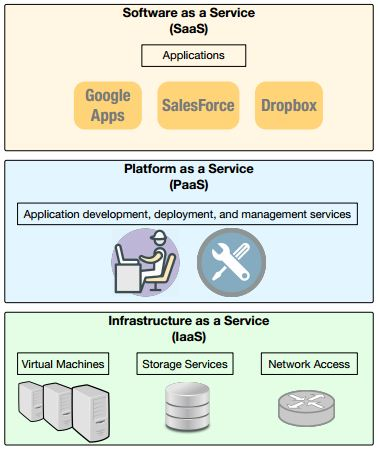
\includegraphics[width=190pt,height=240pt]{figures/cloud-computing.JPG}}\\
%		\caption[Cloud computing service offerings]{\footnotesize \textbf{{Cloud computing service offerings} }}
%\label{fig:ccs}
%\end{center}		
%\end{figure}

\subsection{Versions of Angular}
\hspace{0.2in}Early version of Angular framework was called as AngularJS. Angular 2+ versions are simply called as Angular. It is a completely rewritten version of AngularJS \cite{rewritten}. In this work, Angular refers to the Angular 2+ versions, unless otherwise stated. 

\subsection{Differences in AngularJS and Angular 2+}
Differences between AngularJS and Angular  2+ have stated below.
 
\begin{itemize}
\item{\textbf{ Speed :}  Angular is much faster than AnguarJS. Boot time of Angular applications has been increased by at least 5 times \cite{faster}.}
\item{\textbf{ Architecture :} Angular does not use \$scope or controllers anymore, instead it uses a hierarchy of components. }
\item{\textbf{ Mobile development :} Angular mainly focuses on  performance issues which are issential for running app on a Mobile Platform. }
\item{\textbf{ Modularity :} The core functionality of Angular has been moved to modules, producing a faster, lighter core. }
\item{\textbf{ Language :} Angular uses typescript to write applications, where as AngularJS uses javascript. TypeScript is a superset of JavaScript.}
\item{\textbf{ Improved dependency injection :} Angular used a new Improved Dependacy Injection techniques. }
\end{itemize}



%%::::::::::::::::::::::::::::::::::::::::::::::::::::::::::::::::::::::::::::::::::::::::::::::::::::::::::::::::::::::::::::::
\section{REST}

\hspace*{0.2in}REpresentational State Transfer (REST) \cite{rest} is a set of principles that describes how resources on a server machine are addressed and accessed by  another machine on the same network. The resources (or also called as Web Services) exposed via REST are often called RESTful Web Services. 

Characterization of RESTful Web Services can be given as :
\begin{itemize}
\item{ RESTful Web Services should be stateless \cite{stateless}. }
\item{ Every resource should be uniquly addressable. }
\item{ Access resources over HTTP commands of GET, PUT, DELETE, POST etc. }
\item{ Returned response should in XML or JSON. }
\end{itemize}

\hspace*{0.2in}In RESTful Web Services, every resource is given a URI (Uniform Resource Identifier). A resource can be a file, single record in the database, set of records, a table or the database itself etc. When this resource is requested by a client machine, it is converted into a uniform format (XML or JSON) before sending which can be understood by both machines.  RESTful Web Services are stateless \cite{stateless}. All the session information is stored only in the client machine. Each request from any client carries all the neccessary information to successfully complete the request.

\hspace*{0.2in}SOAP \cite{soap} is another standard as an alternavice for REST but with some differences. SOAP-based Web Services have an official standard, but REST-based Web Services don't.  SOAP is a protocol, but REST is an architectural style. REST is not really a standard but it makes use of other standards such as HTTP, XML, URI, JSON etc.

\subsection{REST Semantics}

\hspace*{0.2in}A RESTful API ( Application Programming Interface ) is simply a collection of URIs ( Uniform Resource Indentifiers ), all HTTP requests to these URIs and some JSON ( XML is also preferred as much as JSON ) representations of resources. These URIs should follow a principal that adheres to REST. Each resource on the server has its own URI or we can also call it an address.

\hspace*{0.2in}For resources residing on the server, nouns should be used as opposed to verbs which describes actions. A RESTful URI should refer to a resource that is a thing instead of referring to an action\cite{restnaming}.

\hspace*{0.2in}Some example of the server resources are given as follows:
\begin{itemize}
\item Users of the bulletin board system.
\item A list of courses taught by a professor.
\item A user's posts over a period of time.
\item An article about global warming.
\end{itemize}

\hspace*{0.2in}Each resource on the server exposing RESTful Web Services will have at least one URI to identify that resource. URIs should follow a predictable, hierarchical structure to enhance understandability and, therefore, usability. This is not a REST rule or constraint, but it keeps the API look better and easier to follow\cite{restnaming}.


Below some examples explained how one should define URIs for server resources:\\

To create a new student on the server:\\
\begin{lstlisting}[language=command]
	POST http://www.example.com/students\\
\end{lstlisting}

To read a student with Student ID 33:\\
GET http://www.example.com/students/33 \\
The same URI can be used for PUT and DELETE, to update and delete, respectively.\\

Here is an example URIs for courses:\\
POST http://www.example.com/courses for creating a new course.\\

GET|PUT|DELETE http://www.example.com/courses/62\\
for reading, updating, deleting course 62, respectively.\\

What if there is a need to apply to new course for a student? One option can be: \\
POST http://www.example.com/courses \\
And that could work to add a course, but it looks like it is outside the context of a student.\\

Because we want to add a new course for a student, this URI doesnt look , as it should be. It could be argued that the following URI would offer better clarity: \\
POST http://www.example.com/students/33/courses \\
Now we know we're adding a new course for Student ID 33.\\

Now what would the following return?\\
GET http://www.example.com/students/33/courses\\
Probably a list of courses for student id 33 has has enrolled. Note: we may choose to not support DELETE or PUT for that url since it's operating on a collection.\\


\section{HTTP}


\hspace*{0.2in}HTTP is very popular Request–-Response protocol in the client–server model in a network. A browser software, for example, could be the client in this model and an application running on a other machine having a website may be the server in this model. The client makes an HTTP request to the server. The server  provides resources such as HTML files and other many types of content, or it performs other tasks on behalf of the client machine, returns a response message to the client. The response received from server contains status information about the sent request and possibly could also contain requested content in its message body.

\subsection{HTTP Methods}

HTTP protocol defines `methods' (sometimes also called as verbs) to indicate the required action that needs to be performed on the identified resource. This resource represents, whether existing data or data that is generated on the fly, relies on the implementation of the server. 

\begin{enumerate}
\item \textbf{GET : } The HTTP GET method is used to read a resource residing on a server. In a successful request, GET returns a response in XML/JSON and an HTTP response code of 200. In case if an error occures , it returns code 4** or 5**, but mostly returns a 404 (404 is a NOT FOUND) or 400 (400 is a BAD REQUEST).

\hspace*{0.2in}GET requests are used only to read resources and not to change them. So, when used this way (i.e without modifiying anything on the server ), they are considered safe. They (requests) can be called without any risk of data modification (or data corruption)—calling it once has the similar effect as calling it 100 times, or none at all. Also, GET is a idempotent request, which means that making multiple similar requests will have the same result as a single very first  request.

Examples:\\
GET http://www.example.com/students/123\\
GET http://www.example.com/students/123/courses\\

\item \textbf{HEAD : } The HEAD method in the HTTP protocol desires for a response similar to that of a GET request, but no response body should be there. This is  very useful for fetching metadata specified in response headers, without having to transport the full content that comes with that request.

\item \textbf{POST : } The POST method in HTTP is mostly used to create new resources on the server. On successful creation of a resourse, it return HTTP response status 201, returning a Location header with a link to the just created resource with the 201 response status.

POST method is neither safe nor idempotent. It is desirable only for non-idempotent resource requests. Making two similar POST requests will mostly result in two resources containing the same type data.

Examples:\\
POST http://www.example.com/students\\
POST http://www.example.com/students/123/courses\\

\item \textbf{PUT : } PUT is used to update the resources residing on server, PUT-ing to a known resource URI with the request body containing the newly-updated resource. PUT can also be used to create new resources, but it is not recommanded. Also, use POST to create new resources and provide the client-defined ID in the body.

\hspace*{0.2in}On successful update operation, it should return 200 status code (or 204 if not returning any content in the body) from a PUT. If PUT used to create, should return HTTP status code 201 on successful creation of the resource. A body in the response is optional. It is optional to return a link in the location header in the creation case since the client already set the resource ID.

\hspace*{0.2in}PUT method is not safe, means it modifies a resource (or creates) state on the server, but it is idempotent. If you create or update a resource residing on the server using PUT method and then make that same request again, the resource is still there and also has the same state as it did with the very first request. If calling PUT on a resource increments a counter  value within the resource residing on the server, the call is no longer said to be idempotent. Many times it happens and it may be enough to document that the call is not idempotent. However, it's recommended to keep PUT requests idempotent.

Examples:\\
PUT http://www.example.com/students/123\\
PUT http://www.example.com/students/123/courses/987\\


\item \textbf{DELETE : } DELETE method in the HTTP protocol is used to delete a resource which is indentified by a URI address. On successful deletion of the resource, it returns HTTP status code 200 ( also called as OK response) with a response body, with a possible wrapped response. Either that or return HTTP status code 204 (called as NO CONTENT) without any response body in the reply. A 204 status code with no body, or the JSON-style response and HTTP status 200 are the recommended responses in this case.

\hspace*{0.2in}DELETE operations are idempotent operations. If you DELETE a resource residing on the server, it's will be removed, if access is granted. Calling DELETE multiple times on that resource ends up the same one: the resource is deleted. If calling DELETE , decrements a counter value, the DELETE call is no longer remains idempotent. Using POST for non-idempotent resource requests is desired and adheres to quality.

\hspace*{0.2in} Calling DELETE method on a resource, more than once will often return a 404 (also called NOT FOUND) since it was already deleted and so it is no longer available to delete. It just no longer exists. This makes DELETE operations no longer idempotent, but the end-state of the resource remains the same. Returning a 404 is ok and communicates well the status code of the request.

Examples:\\
DELETE http://www.example.com/students/123\\
DELETE http://www.example.com/students/123/courses\\


\item \textbf{PATCH : } PATCH is mostly be used for partially modifying resources residing on the server. The PATCH request only needs to contain the changes to the resource, it does not need the complete resource. This is similar to PUT, but the body of the request contains a set of operation that describe how a resource currently residing on the server should be modified to produce a new version of the resource. 

\hspace*{0.2in}PATCH method is neither safe nor idempotent operation. But a PATCH method request can be made in such a way that it looks idempotent, it also helps to  prevent bad outputs that come from collisions between two PATCH requests on the same resource at the same time. Collisions from many PATCH requests may be a lot more dangerous than PUT collisions because some patch formats need to operate from a known base-point. Clients using this kind of patch application hould be using a conditional request such that the request will be failed completely if the resource has been updated since the time that client last accessed the resource. For example, the client can make a use of ETag in an If-Match header on the PATCH request made to the server.

Examples:\\
PATCH http://www.example.com/students/123\\
PATCH http://www.example.com/students/123/courses/987\\

\end{enumerate}

%%::::::::::::::::::::::::::::::::::::::::::::::::::::::::::::::::::::::::::::::::::::::::::::::::::::::::::::::::::::::::::::::
\section{Observables}

\hspace*{0.2in}Observable are a very integral part of Angular. It  is not just specific to  Angular, but it is a popular standard used to manage asyncronous data. Observables allow a continuous stream of communication in which multiple data values can be sent over time. We get a pattern of processing the data by using operations similar to array operations to parse, modify. Angular framework makes use of observables broadly. Mostly used in the HTTP service and the event system of Angular.
	
	
\hspace*{0.2in}In an ordinary method call (which are synchronous), something like this happens:
\begin{enumerate}
\item Call a method.
\item Wait for the method to finish.
\item Store the return value from that method in a variable.
\item Use that variable and its new value to do something useful.
\end{enumerate}

\hspace*{0.2in}In the asynchronous model the flow goes more like this:
\begin{enumerate}
\item Define a method that does some work and returns a value from the asynchronous call
\item Define this asynchronous call as an Observable.
\item Subscribe to this Obervable and provide a method to be called.
\item Continue processing other things; whenever the call returns, the provided method will begin to operate on its return value or values -- the items emitted by the Observable.
\end{enumerate}


In many programming tasks, you more or less expect that the instructions (programs) you write and implement will execute and complete incrementally, one by one, in the order as you have written them. But in some cases, many instructions might execute in parallel and their results are captured afterwards, in random order, by “observers.” Rather than calling a function, you define a technique for fetching and transforming the data, in the form of an “Observable,” and then subscribe to it.

An advantage of this technique is when you have a lot  of tasks that are  independent of each other, you can start them all at the same time rather than waiting for each one to complete before starting the another one. This way your entire all of your tasks only takes as long to complete as the longest task among all tasks.



%%::::::::::::::::::::::::::::::::::::::::::::::::::::::::::::::::::::::::::::::::::::::::::::::::::::::::::::::::::::::::::::::
\section{Data Formats used }

\hspace*{0.2in}JSON, or JavaScript Object Notation, is a minimal, readable format for structuring data. It is used mainly to transmit data between a server and a client, as an alternative to XML. 
		
\hspace*{0.2in}It is a very common data format used for asynchronous client/server communication, including as a replacement for XML in some AJAX-style systems. JSON is a language-independent data format. It was derived from JavaScript, but as of year 2017 many programming languages include code to generate and parse JSON-format data. The official Internet media type for JSON is `application/json'. JSON filenames use the extension `.json'.


\subsection{JSON}

\textbf{What is JSON?}\\
\hspace*{0.2in}JSON, or JavaScript Object Notation, is a minimal, readable format used for structuring data. It is used primarily to send data between a server and web application(or client), as an alternative to XML. 

\textbf{Keys and Values}\\

The two primary properties that are part of JSON are keys and values. 

Key: A key is always a string specified in quotation marks.
Value: A value can be a string, number, boolean value (true or false), array, or object.
Key/Value Pair: A key value pair has a specific syntax, with the key then a colon followed by the value. Key/value pairs are separated by using a comma.
Let's take one line example of JSON and identify each part of the code.

"foo" : "bar"
This example is a key/value pair. The key is "foo" and the value is "bar".

\textbf{Types of Values}\\

Array: An associative array of values.
Boolean: True or false.
Number: An integer.
Object: An associative array of key/value pairs.
String: Zero or more text characters which mostly form a word.

\textbf{Arrays}\\

Array can be used as value in key/value pairs if JSON object. Array is represented by a square brackets, within it all values of array separated by comma.

"foo" : {
  "bar" : "Hello",
  "baz" : [ "quuz", "norf" ]
}

\textbf{Objects}\\

An object is specified by curly brackets. Everything inside of that curly brackets is part of that object. So that means "foo" and the corresponding object are a key/value pair.

"foo" : {
  "bar" : "Hello"
}\\
The key/value pair "bar" : "Hello" is nested inside the key/value pair "foo" : { ... }. \\
That's an example of a hierarchy in JSON data.


\chapter{Literature Review}
\pagestyle{fancy}
\fancyhead[LO]{\itshape\nouppercase{\rightmark}}

\hspace{0.2in} Angular Web Development framework is becoming popular among Web developers everyday. Hundreds of third party modules (also called as libraries or packages) exists for Angular framework. All Angular modules are available as open--source modules on www.npmjs.org. Angular itself is dependent on NodeJS and Node Package Manager (npm), that is, Angular is distributed as a npm package. Users can install angular by following npm command (npm install angular). Similiar way Angular modules are hosted on www.npmjs.org for others to install and use, and also these packages are installed in the same way (npm install `packagename'). This chapter takes survey at similar modules to the one implented by this thesis work, and examines the differences and drawbacks here.

\section{Related Work}

\hspace{0.2in}angular-nested-resource \cite{angular-nested-resource} is an angular module that helps working with RESTful models. It does not have any major dependencies and does not make use of ladash library like other many other libraries do. 
This implementation focuses on the very first version of Angular, that is, AngularJS. Modules implemented for AngularJS and Angular are completly incompatible with each other, as they have a very different architectural styles of their implementation.
angular-nested-resource have implementation based in nested objects. It uses Promises to handle the asynchronus data. \\

\hspace{0.2in} Another popular implementation to  RESTful Web Services for Angular is ngx-restangular \cite{ngx-restangular}. This project is the follow-up of the original Restangular project.ngx-restangular does not support AngularJS, It only supports Angular 2+ versions. This module simplifies HTTP's common methods such as  GET, POST, DELETE, and UPDATE requests. This module can be used for RESTful apps. This module changed its name from ng2-restangular to ngx-restangular because of implementation of Semantic Versioning by Angular's Core Team. NPM (Node Package Manager) name has also changed, and you can install latest version of  this module by execuing npm install ngx-restangular in a command window.\\

\hspace{0.2in} angular2-rest\cite{angular2-rest} is another Angular 2 HTTP client to access the RESTful Web Services. It is implemented in Typescript. This is yet production ready, and it is still in experimental phase (apha phase).\\

\hspace{0.2in} ng2-rest-api\cite{ng2-rest-api} is a HTTP client to consume RESTful Web Services implemented for Angular 2+ versions. It is built on Angular2/http module in the Angular library with TypeScript. It is a  REST API template for all api consumption in an angular application. It's an Angular2 rest template for all CRUD operations (Create, Read, Update and Delete operations). This module has not been published to npm (node package manager), so its only available to  download on githhub, after downloding include it in your service folder. This module does not supports nesting of object, thus have only API of only few functions. Functions available are get(), create(), update(), delete() for HTTP's GET, POST, PUT, DELETE operations respectively. This module has a drawback that you can not configure application wide settings. HTTP headers field has to be set every time a request is made. angular-rest-service (proposed by this thesis work) overcomes this problem by providing application wide settings.
\chapter{Proposed Work}
\pagestyle{fancy}
\fancyhead[LO]{\itshape\nouppercase{\rightmark}}



%%:::::::::::::::::::::::::::::::::::::::::::::::::::::::::::::::::::::::::::::::::::::::::::::::::::::::::::::::::::::::::::::::
\section{Problem Statement}

\hspace{0.2in}This project aims to design and implement a module for Angular to consume RESTful Web Services.
It makes use of Angular's http module to make request over HTTP to a RESTful Web Service and uses HTTP's standard methods such as GET, PUT, POST etc. This module, called hereafter `\textbf{angular-rest-service}', is made available as a npm package on www.npmjs.org.


%%:::::::::::::::::::::::::::::::::::::::::::::::::::::::::::::::::::::::::::::::::::::::::::::::::::::::::::::::::::::::::::::::
\section{Setting Up}

\hspace{0.2in}Angular applications and Angular core itself are dependent on functionalities provided by third parties packages. To install Angular, NodeJS and Node Package Manager (npm) are required. Once NodeJS and npm are installed, Angular can be installed by using npm command line tools. `npm install' requires an active Internet connection. Please set proxy using `npm config' if you are behind proxy.\\
\\
To install angular, execute the following command.
\begin{lstlisting}[language=command]
	 npm install angular
\end{lstlisting}
	  

\subsection{Installing angular-rest-service}

\hspace{0.2in}Once npm is installed, This module can be installed by executing the following command from the command line (or Terminal in case of Linux). Before executing the following command, first go to the root directory of your Angular project.
	
\begin{lstlisting}[language=command]
	npm install angular-rest-service
\end{lstlisting}
	
\hspace{0.2in}After successful execution of the above command, This module should be available into the node module directory. Above command only makes the module accessible to the current project. To make it accessible from anywhere, use the -g or --global flag.
	
\begin{lstlisting}[language=command]
	npm install angular-rest-service -g
\end{lstlisting}
	
\hspace{0.2in}The -g parameter indicates the this module should be installed into global modules directory and should be accessible to all projects.	
	

		
%%:::::::::::::::::::::::::::::::::::::::::::
\subsection{Importing angular-rest-service to your project}

\hspace{0.2in}Import AngularRestServiceModule, AngularRestService and \\AngularRestServiceSettings into your root module. Once imported, add the AngularRestServiceModule to the import's array of the @NgModule metadata. This way all the features from the AngularRestService will accessible to the entire root module of the Angular Project. Add AngularRestService and AngularRestServiceSettings to the providers array of @NgModule metadata.
	
\hspace{0.2in}The updated root module file should look like this:
	
	
\begin{lstlisting}[language=Typescript]
import { BrowserModule } from '@angular/platform-browser';
import { NgModule } from '@angular/core';
import { AppComponent } from './app.component';

import {AngularRestServiceModule, AngularRestService, AngularRestServiceSettings} from 'angular-rest-service';

@NgModule({
  declarations: [   AppComponent  ],
  imports: [
    BrowserModule,
    AngularRestServiceModule
  ],
  providers: [AngularRestService, AngularRestServiceSettings],
  bootstrap: [AppComponent]
})
export class AppModule { }

\end{lstlisting}



\hspace{0.2in}Before any request  is made to a resource on the server machine, the base URL of the server machine need to be set.
This Base URL is used for all requests except where custom base URL for the resource is specified. To set the base URL , import the AngularRestServiceSettings into the main component of root module.  Add the AngularRestServiceSettings to the constructor of the component.

\hspace{0.2in}The updated main component should look like this:


\begin{lstlisting}[language=Typescript]
import { Component, OnInit } from '@angular/core';
import { AngularRestServiceSettings } from 'angular-rest-service';

@Component({
  selector: 'app-root',
  templateUrl: './app.component.html',
  styleUrls: ['./app.component.css']
})
export class AppComponent implements OnInit {

	constructor( private settings: AngularRestServiceSettings) { }

  	ngOnInit() {
		this.settings.setBaseUrl("http://base/url/api");
  	}
}
\end{lstlisting}



%%:::::::::::::::::::::::::::::::::::::::::::::::::::::::::::::::::::::::::::::::::::::::::::::::::::::::::::::::::::::::::::::::
\section{angular-rest-service API}

\hspace{0.2in}angular-rest-service module defines a simple inteface, to perform CRUD operations (Create, Read, Update, Delete) on the resources which are exposed via REST. This functions can be accessed by a singleton object which is available to all components that imports AngularRestServiceModule. 
	
	
\begin{enumerate}

\item{
	\textbf{list}(name: string, params?: any): any \\
	This function takes a resource name (eg. users, books, cources, categories etc.)  and some optional parameters. This functions return an object (a list of users or list or books etc.) on which you can perform CRUD operations. To perform this operations, functions such as doGet() or doPost() made available, which uses corresponding HTTP method to perform neccessary operations on these resources.
	
\begin{lstlisting}[language=Typescript]
this.rest.list('users').doGet().subscribe(result=> 
	/* process the result here */ );
\end{lstlisting}
	
}
\item{
	\textbf{filterById}(id: number): any \\
	\hspace{0.2in} filterById() can be used after list(), which is useful when whole list needs to be filtered by given id. E.g. If among all users, a single user with id 23 needs to fetched, following single line code will do the job.
	
\begin{lstlisting}[language=Typescript]
this.rest.list('users').filterById(23).doGet().subscribe(result=> 
	/* process the result here */ );
\end{lstlisting}
	
}
\item{
	\textbf{filterById}(ids: Array): any \\
	\hspace{0.2in} Sometimes fetching several users is required. Overloaded filterById() also takes an array of numbers as input, which are a list of ids of users that needs to be fetched. E.g. If among all users, users with ids 23, 45, 12 needs to fetched, following single line code will do the job.
	
\begin{lstlisting}[language=Typescript]
this.rest.list('users').filterById( [23, 45, 12] )
	.doGet().subscribe(result=> /* process the result here */);
\end{lstlisting}
	
}

\item{
	\textbf{doGet}(): Observable $<$any$>$ \\
	The doGet() function performs a GET request and returns an Observable. As fetching data on a network can take time, these methods needs to asynchronous. Observable are a popular way to handle asynchronous events in Javascript. Observable have a subscribe() method with user defined function as parameter, this function is called as soon as a response received.
}
\item{
	\textbf{doPost}(data  : string): Observable $<$any$>$ \\
		The doPost() function performs a POST request and returns an Observable.For doPost(), a single parameter is required which is a JSON object. This JSON object's format should adhere to the server's RESTful Web Service specification. Once this function is succesfully executed, a new record will be created on the server.
}
\item{
	\textbf{doPut}(data : string ): Observable $<$any$>$ \\
	The doPut() function performs a PUT request and returns an Observable. For doPut(), a single parameter is required which is a JSON object. An id property with a valid value is mandatory to indentify a resource on the server. This JSON object's format should adhere to the server's RESTful Web Service specification. Once this function is succesfully executed, a record with specified id will be upadated on the server.
}
\item{
	\textbf{doDelete}(): Observable $<$any$>$ \\
	The doDelete() function performs a DELETE request and returns an Observable. The URL should locate a valid resource. After the successful execution of this function, returned Observable contains informations about whether the resource successfully deleted or not.
	
}	
\item{
	\textbf{doPatch}(data : string ): Observable $<$any$>$ \\
	
}
\item{ \textbf{addHttpHeader}(name : string, value : string) \\
	Use this function, when there is need to add a http header field in the current request. It should be a valid header field, and the user must have access the set a perticular header field. Some header fields (e.g.  `Accept-Encoding') are not allowed to be set. Only browsers can set these fields. A list of headers fields is maintained for each request. This function adds this header field to the list of already existing header fields. If the header field with same name already exists, its value is overwritten, else a new key--value pair is created. Apart from this, there a global headers list stored in the AngularRestServiceSettings's object. These headers fields are included in each request to the server. If this function specifies a header field that already exists in the global headers, this local value is used instead for the current request.
}
\item{ \textbf{removeHttpHeader}(name : string, value : string) \\
	This function removes a header field from the list of headers fields,  if it already exists. A separate copy of header fields is maintained for each request. 
}
\item{
	\textbf{setParameter}(name : string, value : any) \\
	The setParamter() is used to add a key--value pair in the request url. This function sets the parameter only for the current request. 
	For example:

\begin{lstlisting}[language=Typescript]
let users = this.rest.list("users");
users.setParameter("transform", 1);
    
//makes a /GET request to baseurl/users?transform=1
users.doGet().subscribe(
     response => {
        this.userlist = response.json().users;
     } 
   );
\end{lstlisting}
If user want a parameter to be included in every request, another function is defined in the AngularRestServiceSettings.  

}



\end{enumerate}

	
	
	
	
	
%%:::::::::::::::::::::::::::::::::::::::::::::::::::::::::::::::::::::::::::::::::::::::::::::::::::::::::::::::::::::::::::::::
\section{Module Configuration}


	Module configuraton focuses on changing the behavior of the angular-rest-service. Sometimes the module needs to to congured, e.g. If every request should contaian authentication information in the HTTP header, such information can be set in the AngularRestServiceSettings. Module Configuration contains some functions that used to set application wide settings. AngularRestServiceSettings contains functions that are required to change the behavior of other functions, e.g setting the base url to which all calls should be made or a url paramter that every should made should contain. 
	
\begin{itemize}

\item{ \textbf{setBaseUrl}(base : string) \\
	All request made to a RESTful Web Service have a unique URL or can also be called as Base URL which is common prefix for all resource addresses. The setBaselUrl() function can be used to set the base url which is used in all calls (except a few where Base URL is specified itself as a function parameter) to a RESTful Web Service. \\
	eg. http://abc.xyz/rest/api/ is valid base url.

}
\item{ \textbf{getBaseUrl}() : string \\
	This function returns the currently set Base url. If the Base URL is not set, it simply returns `undefined'.
}
\item{ \textbf{addHttpHeader}(name : string, value : string) \\
	Use this function, when there is need to add a http header field for all requests. It should be a valid header field, and the user must have access the set a perticular header field. Some header fields (e.g.  `Accept-Encoding') are not allowed to be set. Only browsers can set these fields. A list of headers fields is maintained which are included in all requests. This function adds this header field (key--value pair) to the list of already existing global header fields. If the header field with same name already exists, its value is overwritten, else a new key--value pair is created. Apart from this, there a local headers list for each request. These headers fields are included in each request to the server. If this function specifies a header field that already exists in the local headers, this local value is used instead for the current request.
}
\item{ \textbf{removeHttpHeader}(name : string, value : string) \\
	This function removes a header field from the list of global headers fields,  if it already exists. Once this key--value pair is removed from this list, request made after this will not contain this key-value.
}
\item{ \textbf{setGlobalParameter}(name : string, value : string) \\
	Global parameters are a way to maintain a list of key--value pairs, which are required in every request. For example, If request to the server needs to have an api--key to authenticate the user, it will cumbersome to independently add a parameter spearatly for every request. To solve this issue, just set the parameter using this function. Once parameter is successfully set, all request will include the this parameter. 
}

\end{itemize}

	








%%:::::::::::::::::::::::::::::::::::::::::::::::::::::::::::::::::::::::::::::::::::::::::::::::::::::::::::::::::::::::::::::::
\section{Example application}

\hspace{0.2in}Assume we have a server machine exposing RESTful Web Services. We want to fetch a list of all users. The following example shows how to get list of all users and set it to a local variable inside the Angular component. 
Import the angular-rest-service module and complete the basic set up (as explained in previous sections) to start using this module in your Angular project.

\hspace{0.2in}This example makes a GET request to /users expects a response in json format. This response is converted into a json object by using json() method. 

\begin{lstlisting}[language=Typescript]
import { Component, OnInit } from '@angular/core';
import { AngularRestService } from 'angular-rest-service';

@Component({
  selector: 'app-user-list',
  templateUrl: './user-list.component.html',
  styleUrls: ['./user-list.component.css']
})
export class UserListComponent implements OnInit {
  userlist;

  constructor(private rest: AngularRestService) { }

  ngOnInit() {
    let users = this.rest.list("users").doGet().subscribe(
      response => {
        this.userlist = response.json();
      } 
    );
  }
}
\end{lstlisting}

Following example makes a GET request to /users/23.

\begin{lstlisting}[language=Typescript]
let user = this.rest.list("users").filterById(23).doGet().subscribe(
      response => {
        //response.json() hold the user information with id 23;
      });
\end{lstlisting}

POST method is used to create new resources on the server.\\
Following example makes a POST request to /users. The doPost() fuction expects a single parameter in json format.
\begin{lstlisting}[language=Typescript]
let user= {
	"username" : "Vijay",
	"age" : 23,
	"gender" : ''Male''
};

this.rest.list("users").doPost(user).subscribe(res => 
	//res.json() contains info whether a new user created or not
);
\end{lstlisting}


To update a user information : \\
This will to PUT to /users \\
Note that id property is neccessary and should be a number.
\begin{lstlisting}[language=Typescript]

let user = {
	"id" : 23,
	"username" : ''Mayur''
	''gender'' : ''Male''
};
this.rest.list("users").doPut(user).subscribe(res => 
	//res.json() contains info whether a user udpated or not
);
\end{lstlisting}


To delete a user : \\
It makes DELETE request to /users/23.
 \begin{lstlisting}[language=Typescript]
this.rest.list("users").filterById(23).doDelete().subscribe(res => 
	//res.json() contains info whether the user with id deleted or not
);
\end{lstlisting}










%%:::::::::::::::::::::::::::::::::::::::::::::::::::::::::::::::::::::::::::::::::::::::::::::::::::::::::::::::::::::::::::::::
%\section{Handling Authentication}








\chapter{Conclusion}
\pagestyle{fancy}
\fancyhead[LO]{\itshape\nouppercase{\rightmark}}

\hspace{0.2in} This project designed and implemented an Angular module to access RESTful Web Services. This module makes communicating with a REST-based Web Service simpler and in fewer lines of code. It takes care of the authentication, erros, URL construction.  It makes use of Angular's http module to make request over HTTP to a RESTful Web Service and uses HTTP's standard methods such as GET, PUT, POST etc. This module `\textbf{angular-rest-service}' is made available as a npm package on www.npmjs.org. This module can be installed in an Angular by executing `\textbf{npm install angular-rest-service}' from command line, which will download the latest version into the projects' nodule-modules directory. angular-rest-service suppports Basic (or Bearer) authentication, OAuth2 authentication methods. In the future work, additional authentication techniques can be added. 


%% --------------------------------------------------------------------------------------------------APPENDIX
% Now begin the Appendices, including them as separate files
%\appendix % Cue to tell LaTeX that the following 'chapters' are Appendices
%\backmatter

%% -------------------------------------------------------------------------------------------------BIBLOGRAPHY
%\lhead{\emph{Bibliography}}  % Change the left side page header to "Bibliography"
\nocite{hhsa}
\nocite{*}
\bibliographystyle{unsrt}  % Use the "unsrtnat" BibTeX style for formatting the Bibliography
\bibliography{bib}  % The references (bibliography) information are stored in the file named "Bibliography.bib"


\end{document}  % The End